%!TEX root = main.tex


\begin{figure}
	\centering
	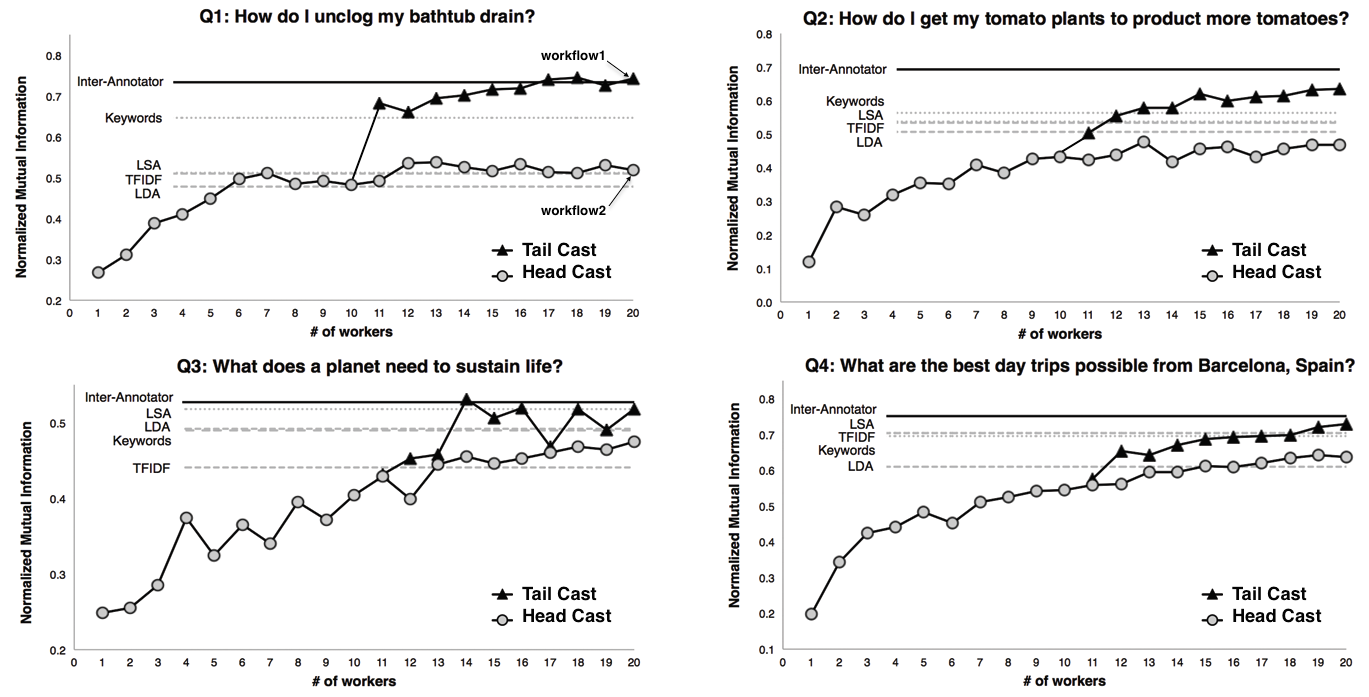
\includegraphics[width=1\columnwidth]{images/numberOfTurkers.png}
	\caption{Perfomance comparison of using diferent number of crowdworkers in Head Cast and Tail Cast.}
	\label{fig:numberOfTurkers}
\end{figure}

\begin{table}
  \centering
% question, number of sources, number of clips, number of turkers
  \begin{tabular}{ c r r r r r r r }
    \hline
	\tabhead{Questions} &
	\tabhead{Inter-annotator} &
	\tabhead{System A} &
	\tabhead{System AB} &
	\tabhead{TF-IDF Baseline} &
	\tabhead{Keywords Baseline} &
	\tabhead{LSA Baseline} &
	\tabhead{LDA Baseline} \\
    \hline
	% 102
	\textbf{Q1} & .7335 & .5190 & \textbf{.7415} & .5099 & .6465 & .5118 & .4780 \\

	% 115 - 2
	\textbf{Q2} & .6928 & .4691 & \textbf{.6347} & .5339 & .5621 & .5373 & .5063 \\

	% 96
	\textbf{Q3} & .4768 & .4247 & \textbf{.4680} & .3901 & .4397 & .4674 & .4417 \\

	% 116
	\textbf{Q4} & .5673 & .6333 & \textbf{.7272} & .6728 & .6762 & .7038 & .6028 \\

	% 137 carbon footprint
	\textbf{Q5} & .6303 & .? & ? & .? & .? & .? & .? \\

	% 139
	\textbf{Q6} & .? & .? & ? & .? & .? & .? & .? \\
    \hline
  \end{tabular}
  \caption{Normalized Mutual Information scores for different systems}
  \label{tab:results}
\end{table}


\subsection{Evaluation Results}

As shown in Table \ref{tab:results}, the full system with both Head Cast and Tail Cast.
performed the best in all four questions with NMI scores
significantly higher than Workflow 1 and the baselines based on word
vector similarity.  It suggests that using crowdworkers to refine outputs from
a machine learning model can be more effective and efficient than simply hiring
more crowdworkers to increase the size of the training set. Of the four
baselines, LSA performed the best.  The Keywords Baseline based on highlights from the crowd
consistently outperformed the TF-IDF Baseline based on all words, it
shows that the crowdworkers are extracting keywords in Head Cast that are
salient for identifying clusters each dataset.

In Figure \ref{fig:numberOfTurkers}, we show the performance of Workflow 1 and
Workflow 2 employing different number of crowdworkers.  Initially, increasing the
number of training data in Head Cast showed significant performance improvement.
After gathering training data from around ten crowdworkers, the amount of performance
gain from hiring additional crowdworkers decreases notable. However, the
results also showed that even with only a few crowdworker in Tail Cast to refine
the clusters from Head Cast, can have further improve the performance significantly. Finally,
with twenty crowdworkers, the system with 10 crowdworkers in each Cast
consistently outperforms having all 20 crowdworkers in Head Cast.

The results showed that the complete System AB can produce clusters with NMI
difference to the gold-standard clusters close to the NMI difference between
the two annotators. Although this does not necessary mean the system produces
near expert results, it suggests that the output is comparable to one produced
by the annotators, who have a global view of the datasets while labeling.

